
\chapter{Introduction to data}
\label{introductionToData}

\section{Data basics}
\label{dataBasics}

%Statistics revolves around using information to make conclusions. Observations or information that is recorded is often called \term{data}.

\subsection{Observations, variables, and possums}

Table~\ref{possumDF} displays rows 1, 2, 3, and 104 of a data set concerning Australian bushtail possums. These observations (measurements) of 104 possums will be referred to as the \data{possum} data set.
\begin{table}[ht]
\begin{center}
\begin{tabular}{ccc ccc cc}
  \hline
& pop & sex & age & headL & skullW & totalL & tailL \\
  \hline
1 & Vic & m & 8 & 94.1 & 60.4 & 89.0 & 36.0 \\
2 & Vic & f & 6 & 92.5 & 57.6 & 91.5 & 36.5 \\
3 & Vic & f & 6 & 94.0 & 60.0 & 95.5 & 39.0 \\
$\vdots$ & $\vdots$ & $\vdots$ & $\vdots$ & $\vdots$ & $\vdots$ & $\vdots$ & $\vdots$ \\
104 & other & f & 3 & 93.6 & 59.9 & 89.0 & 40.0 \\
   \hline
\end{tabular}
\end{center}
\caption{Measurements related to seven variables are provided for each possum.}
\label{possumDF}
%  xtable(possum[c(1,2,3,104), c(1, 3, 4, 5, 6, 7, 8, 9)], digits=1)
\end{table}

Each row relates to a single possum or \term{observation}, and contains that individual possum's measurements for seven variables. For example, Possum 104 is a 3 year old female.
\begin{figure}[tb]
   \centering
   \includegraphics[height=2.8in]{ch1/possumPic/possumPic.jpg}
   \caption{The common brushtail possum of Australia. Photocredits: wollombi on Flickr ({\small http://flickr.com/photos/wollombi/58499575/}).}
   \label{possumPic}
\end{figure}

Each column of Table~\ref{possumDF} represents an attribute known about each observation, and these attributes are called \term{variables}. For instance, the \var{age} variable holds the age about every observed possum in the data set. Descriptions of all of these variables are given in Table~\ref{possumVariables}.
\begin{table}[ht]
\begin{center}\small
\begin{tabular}{lp{10.5cm}}
\hline
{\bf variable} & {\bf description} \\
%\hspace{0.5cm} \= \var{case}: ID number associated with the possum (\resp{1}, \resp{2}, ..., \resp{104}) \\
%\> \var{site}: the location where each possum was trapped (\resp{1}, \resp{2}, ..., \resp{7}) \\
\hline
\var{pop} & the location where the possum was trapped (\resp{Vic} or \resp{other}) \\
\var{sex} &the possum's gender (\resp{m} or \resp{f}) \\
\var{age} & age, in years (positive whole number, data ranges between \resp{1} and \resp{9}) \\
\var{headL} & head length, in mm (positive number, data range: \resp{82.5} to \resp{103.1}) \\
\var{skullW} & skull width, in mm (positive number, data range: \resp{50.0} to \resp{68.6}) \\
\var{totalL} & total length, in cm (positive number, data range: \resp{75.0} to \resp{96.5}) \\
\var{tailL} &tail length, in cm (positive number, data range: \resp{32.0} to \resp{43.0}) \\
%\> \var{earConch}: 
\hline
\end{tabular}
\end{center}
\caption{Variables and their descriptions for the \data{possum} data set.}
\label{possumVariables}
\end{table}

In practice, it is especially important to ask clarifying questions to ensure important aspects of the data are understood. For instance, a possum trapped in Victoria would have \var{pop} = \resp{Vic} while a possum trapped in New South Wales or Queensland would have \var{pop} = \resp{other}.

\subsection{Variable relationships}
\label{variableRelations}

In practice, relationships between the variables are typically of interest. Questions about the \data{possum} data set include
\begin{enumerate}
\item[(1)] If a possum has a shorter-than-average head, do you think its skull width will be smaller or larger than the average skull width? \label{possumHeadSizeQuestion}
\item[(2)] Will males or females, on the average, be longer? \label{possibleCausationQuestionForPossums}
\item[(3)] Which population of possum will be larger on the average: \resp{Vic} or \resp{other}?
\item[(4)] Does the proportion of males differ based on location, i.e. from \resp{Vic} to \resp{other} in the \var{pop} variable?
\end{enumerate}

\begin{exercise} \label{4possumQuestions}
Give an answer (guess) to each of the questions above without examining the data\footnote{Exercises scattered throughout this chapter are generally informal and are intended to be very brief. Questions at the end of the chapter are more formal and will require more thought.}.
\end{exercise}

\begin{exercise}
How confident are you about your answers in Exercise~\exer{4possumQuestions}?
\end{exercise}

Number crunching could answer each of the four questions about \data{possum}; however, it might be more interesting and perhaps even more obvious by examining graphs of the data.
\begin{figure}[hbt]
   \centering
   \includegraphics[height=2.5in]{ch1/possumHeadVsSkullW/possumHeadVsSkullW}
   \caption{A scatterplot showing \var{skullW} against \var{headL}. The first possum with a head length of 94.1mm and a skull width of 60.4mm is darkened for instructive purposes.}
   \label{possumHeadVsSkullW}
\end{figure}

Scatterplots are graphs used to study the relationship between two variables. Figure~\ref{possumHeadVsSkullW} compares \var{headL} and \var{skullW}. Each point represents a single possum. For instance, the red dot corresponds to Possum 1 from Table~\ref{possumDF}, which has a head length of 94.1mm and a skull width of 60.4mm. The scatterplot suggests that if a possum tends to have a short head, then the skull width also tends to be smaller. That is, if a possum has a smaller value of \var{headL}, the possum also tends to have a smaller skull width. \\

\begin{exercise}
Create two additional questions about the relationships between the variables that are of interest to you.
\end{exercise}

%The first question about \data{possum}, discussed above, is sort of boring. So possums with short heads tend to have slimmer skulls -- that isn't surprising! But some of the other questions might stem from a deeper question.

\section{Data format, collection, and properties}

\subsection{Data Matrix}

The data in Table~\ref{possumDF} represent a \term{data matrix}\footnote{In R, a data matrix is called a \term{data frame}.}. This is a common organization format for data. Each row of a data frame represents a separate observation and each column represents a variable.

The data matrix called \data{Cars} is shown in Table~\ref{carsDF}. Cars 1, 2, and 54 are shown with six variables: \var{type}, \var{price}, \var{mpgCity}, \var{driveTrain}, \var{passengers}, and \var{weight}, shown in Table~\ref{carsVariables}.
\begin{table}[ht]
\begin{center}
\begin{tabular}{c ccc ccc}
  \hline
 & type & price & mpgCity & driveTrain & passengers & weight \\
  \hline
1 & Small & 15.9 & 25 & Front &  5 & 2705 \\
  2 & Midsize & 33.9 & 18 & Front &  5 & 3560 \\
$\vdots$ & $\vdots$ & $\vdots$ & $\vdots$ & $\vdots$ & $\vdots$ & $\vdots$ \\
  54 & Midsize & 26.7 & 20 & Front &  5 & 3245 \\
  \hline
\end{tabular}
\end{center}
\caption{The \data{Cars} data matrix.}
\label{carsDF}
\end{table}
\begin{table}[h]
\begin{center}\small
\begin{tabular}{lp{10.5cm}}
\hline
{\bf variable} & {\bf description} \\
\hline
\var{type} & car type (\resp{small}, \resp{midsize}, or \resp{large}) \\
\var{price} & the average purchase price of the vehicles in \$1000's (positive number) \\
\var{mpgCity} & rated city mileage in miles per gallon (positive number) \\
\var{driveTrain} & the drive train (\resp{front}, \resp{rear}, \resp{4WD}) \\
\var{passengers} & passenger capacity (positive whole number, taking values \resp{4}, \resp{5}, or \resp{6}) \\
\var{weight} & car weight in pounds (positive number) \\
\hline
\end{tabular}
\end{center}
\caption{Variables and their descriptions for the \data{Cars} data set.}
\label{carsVariables}
\end{table}

\subsection{Sampling}

The \data{Cars} data set represents a \term{sample} of cars from 1993. All cars from 1993 represent the \term{population}, and the cars in the sample were \term{randomly} selected from the population.
\begin{figure}[h]
\centering
\includegraphics[height=1.5in]{ch1/popToSample/popToSample}
\caption{Cars from the population are randomly selected to be included in the sample.}
\label{popToSample}
\end{figure}
Randomly selected in this context is equivalent to a raffle to select cars. The name of each car was written on a raffle ticket, and 54 tickets were drawn.

\subsection{Random samples and bias}

Why pick a sample randomly? Suppose the cars were just picked by whatever cars were of greatest interest to the person doing the picking. \\

\begin{exercise}
If you were collecting the data, what kind of cars would you be interested in including? Would everyone share this interest?
\end{exercise}

David is interested in high mileage, so he might intentionally or accidentally pick mostly cars with the best mileage. One type of car might be favored over another. This favoratism, accidental or intentional, introduces \term{bias} into a sample.
\begin{figure}[h]
\centering
\includegraphics[height=1.5in]{ch1/popToSample/popToSubSample}
\caption{Instead of sampling from all cars from 1993, David samples only cars with high mileage.}
\label{popToSubSample}
\end{figure}
Sampling randomly helps resolve this problem. The most basic random sample is called a \term{simple random sample}, and is the equivalent of using a raffle to pick the sample. This means that everyone in the population has an equal chance of being included in the sample and there is no implied connection between the individuals in the sample. The simple act of taking a simple random sample helps eliminate bias but does not always solve the problem completely.

Even when people are seemingly picked at random (for surveys, etc.), caution must be exercised if the \term{non-response} is high. For instance, if only 15\% of the people randomly sampled for a survey actually respond, then it is unclear whether the results are \term{representative} of the rest of the population of interest. \term{Non-response bias} can skew results one way or another\footnote{In major polling outfits such as Gallup, researchers try to keep the non-response level low while also making corrections to attempt to offset any lingering bias. These types of corrections are beyond the scope of this text.}.
\begin{figure}[h]
\centering
\includegraphics[height=1.5in]{ch1/popToSample/surveySample}
\caption{Surveys may result in only reaching a certain group within the population, and it is not obvious how to fix this problem.}
\label{surveySample}
\end{figure}

Another common downfall is a \term{convenience sample}, where the individuals observed were easily accessible and so more likely to be included in the sample. For instance, if a political survey is done by stopping people walking in the Bronx, this probably will not fairly represent all of New York City. It is often difficult to discern what sub-population a convenience sample represents. \\

\begin{exercise}
If you stand outside your school's student union to survey people who walk by, what sub-population do you think you are sampling? How would this sub-population be different from the population of the city?
\end{exercise}

\subsection{Independence}

There was no connection between which cars were or were not selected for the \data{Cars} data set. They were \term{independently} selected. More formally, these observations are said to be \term{independent} of each other. Independence is a key concept in statistics.

It is also possible for variables to be independent of one-another. If knowing a car's city mileage provided no information about its price, then \var{mpgCity} and \var{price} are independent variables. \\

\begin{termBox}{\tBoxTitle{Independence}
Two things are independent of each other if they have no bearing or effect on each other.}
\end{termBox}

The variables \var{mpgCity} and \var{price} can be independent, and the observations car 35 and car 51 can be independent; however, the variable \var{price} cannot be independent of car 45. In statistics, for two things to be independent of each other, they must be the same type. % ZZQ: reread this paragraph. acceptable?

Even when observations are not explicitly selected at random, such as in the \data{possum} data set, it is often assumed they are independent. Each possum might be equally likely to be caught in the trap, so the trapping itself was used to simulate the random sample. One should always be cautious of these assumptions.

\subsection{Variable types}

Examine each of the following variables in the \data{Cars} data set: \var{type}, \var{price}, \var{driveTrain}, and \var{passengers}. Each of these variables is inherently different from the others yet many of them share characteristics.

First consider \var{price}, which is said to be a \term{numerical} variable since the values it takes are number \emph{and} those numbers have an inherent ordering. That is, all 50 cars could be ordered from most expensive to least expensive or vice-versa, and ties are okay.

The \var{passengers} variable is also numerical, although it seems to be a little different than \var{price}. The variable \var{passengers} can only take whole positive numbers (\resp{1}, \resp{2}, ...) since there isn't a way to have 4.5 passengers. The variable \var{passengers} is said to be \term{discrete} since it only can take numerical values with jumps (e.g. 1, 2, 3, ...). On the other hand, \var{price} is said to be \term{continuous}. % ZZQ: the definition of discrete needs work

The variable \var{driveTrain} can only take a few different values: \resp{front}, \resp{rear}, and \resp{4WD}. Because the responses themselves are categories, \var{driveTrain} is called a \term{categorical} variable\footnote{Sometimes also called a \term{nominal} variable.}. The  three possible values (\resp{front}, \resp{rear}, \resp{4WD}) are called the \term{levels} of \var{driveTrain}.

Finally, consider \var{type}, which seems to be some sort of hybrid: it is a categorical variable but there is some inherent ordering: \resp{small} $<$ \resp{midsize} $<$ \resp{large}. A variable with these properties is called an \term{ordinal} variable. To simplify analyses, any ordinal variables in this book will be treated as categorical variables.
\begin{center}
\includegraphics[height=1.5in]{ch1/variables/variables}
\end{center}

\begin{example}{Examine the types of variables from the data set \data{possum}.}
Because the \var{sex} variable takes non-numerical values, it is a categorical variable. Because \var{headL} has numbers as a response and these numbers can be ordered, it is a numerical variable. More specifically, since \var{headL} can be any length, this variable is a \emph{continuous} numerical variable even though the measured values are all rounded to one decimal.
\end{example}

\begin{exercise}
Identify each of the remaining variables in the \data{possum} data set as either continuous numerical, discrete numerical, or categorical.
\end{exercise}

\begin{exercise}\label{possumSiteExer}
An additional variable was recorded for the \data{possum} data set called \var{site}. This \var{site} variable was a number \resp{1}, \resp{2}, ..., \resp{7}, however, the ordering of the numbers doesn't actually hold meaning. Is this a numerical or categorical variable? Answer in the footnote\footnote{Because the order of the numbers holds no meaning, this is a categorical variable.}.
\end{exercise}


\section{Examining numerical data}
\label{numericalData}

\subsection{Scatterplots for paired data}
\label{scatterPlots}

Scatterplots provide an observation-by-observation view of data for two numerical variables. In Section~\ref{variableRelations}, a scatterplot was informally introduced and used to examine how head length and skull width were related in the \data{possum} data set. Another scatterplot is shown in Figure~\ref{carsPriceVsWeight}, comparing \var{price} and \var{weight} for the \data{Cars} data set.
\begin{figure}[bth]
   \centering
   \includegraphics[height=2.6in]{ch1/carsPriceVsWeight/carsPriceVsWeight}
   \caption{A scatterplot of \var{price} versus \var{weight} for the \data{Cars} data set.}
   \label{carsPriceVsWeight}
\end{figure}

In any scatterplot, each point represents a single observation. Since there are 54 observations in \data{Cars}, there are 54 points in Figure~\ref{carsPriceVsWeight}. \\

\begin{exercise}
How are scatterplots useful?
\end{exercise}

\subsection{Association}

The data in Figure~\ref{carsPriceVsWeight} appear to follow some \term{trend}. That is, the average price for a car tends to be larger when the vehicle weight is larger (and vice-versa). Variables with this type of relationship are said to be \term{associated} with one-another. If an increase in one variable is associated with an increase in the other as in Figure~\ref{carsPriceVsWeight}, then it is a \term{positive association}. If the increase in one variable is associated with a decrease in the other such as in Figure~\ref{carsMpgCityVsWeight}, then the variables are \term{negatively associated}. Some associations are more linear, like relationship
between mpgCity and weight, shown in Figure~\ref{carsMpgCityVsWeight}. Others, like the one seen in Figure~\ref{carsPriceVsWeight}, can be curved.
\begin{figure}[bth]
   \centering
   \includegraphics[height=2.6in]{ch1/carsMpgCityVsWeight/carsMpgCityVsWeight}
   \caption{A scatterplot of \var{mpgCity} versus \var{weight} for the \data{Cars} data set. Since an increase in one variable typically means the other tends to drop (in the data), they are negatively associated variables.}
   \label{carsMpgCityVsWeight}
\end{figure} \\

\begin{exercise}
Make a scatterplot of two variables that would have a horseshoe shape.
\end{exercise}

When variables are associated with each other, they cannot be independent. The reverse is also true: two variables that are independent are not associated with each other. \\

\begin{termBox}{\tBoxTitle{Associated or independent, not both}
A pair of variables are either related in some way (associated) or not (independent). No pair of variables is both associated and independent.}
\end{termBox}

Association between categorical variables will be discussed in Section~\ref{categoricalData}, and associations between categorical and numerical variables will be discussed in Section~\ref{comparingAcrossGroups}.

\subsection{Dot plots and the mean}
\label{dotPlot}

Sometimes two variables is one too many: sometimes only one variable is of interest. In these cases, a dot plot provides the most basic of displays. A dot plot is basically a one-variable scatterplot.
\begin{figure}[bth]
   \centering
   \includegraphics[height=1.3in]{ch1/carsPriceDotPlot/carsPriceDotPlot}
   \caption{A dot plot of \var{price} for the \data{Cars} data set. The triangle marks the sample's mean price.}
   \label{carsPriceDotPlot}
\end{figure}

The \term{mean}, sometimes called the average, is a way to measure the center of a \term{distribution} of data. To find the mean price of the cars, add up all the prices in the sample and divide by the number of observations.
\begin{eqnarray}
\bar{x} = \frac{15.9 + 33.9 + \cdots + 26.7}{54} = 19.99259
\label{sampleMeanEquation}
\end{eqnarray}
The sample mean is often labeled $\bar{x}$. The letter $x$ is being used as an abbreviation for \var{price}, and the bar says it is the sample average of price. \\

\begin{termBox}{\tBoxTitle{Mean}
The sample mean of a numerical variable (continuous or discrete) is computed as the sum of all of the observations divided by the total number of observations:
\begin{eqnarray}
\bar{x} = \frac{x_1+x_2+\cdots+x_n}{n}
\label{meanEquation}
\end{eqnarray}
where $x_1, ..., x_n$ represent the $n$ observed values.}
\end{termBox}

\begin{exercise}
Examine equations~(\ref{sampleMeanEquation}) and~(\ref{meanEquation}). What does $x_1$ correspond to? And $x_2$? Can you infer a general meaning to what $x_i$ might represent. Answers in the footnote\footnote{$x_1$ corresponds to the first observation (15.9), $x_2$ to the second observation (33.9), and $x_i$ would correspond to the $i^{th}$ observation.}.
\end{exercise}

\begin{exercise}
What was $n$ in the \data{Cars} data set? Answer in the footnote\footnote{The sample size is $n=54$.}.
\end{exercise}

The \emph{population} mean is also computed in the same way, however, it has a special label: $\mu_x$. The symbol, $\mu$, is the Greek letter \emph{mu} and tells you that you are considering a population average. \\

\begin{exercise}
Can you determine the exact average price of cars from 1993? (No!) How would you use the data to estimate the average price of all cars from 1993? Answer in the footnote\footnote{The sample mean provides an estimate of the mean price of all cars from 1993.}.
\end{exercise}

%\begin{termBox}{\tBoxTitle{}
%}
%\end{termBox}

The accuracy of a sample estimate -- for instance, how close sample mean $\bar{x}$ is to $\mu_x$ -- is a major topic in this book and will be discussed in detail in Chapters~\ref{foundationsForInference} and~\ref{classicInference}.

\subsection{Histograms and shape}

%\subsubsection{Histogram}

Dot plots show the exact value for each observation. This is great for small data sets, but can become problematic for larger samples. For this reason, it is useful to \emph{bin} the data. For example, create a table of counts for the number of observations between \$5,000 and \$10,000, then the number between \$10,000 to \$15,000, and so on. Observations that fall on the boundary of a bins (e.g. \$10,000), are allocated to the lower bin. This tabulation is shown in Table~\ref{binnedCarsPriceTable}. To make the data easier to see visually, these binned counts are plotted as a bar chart in Figure~\ref{carsPriceHist}. This type of plot is called a \term{histogram}.
\begin{table}[ht]
\begin{center}\small
\begin{tabular}{ccc ccc ccc}
  \hline
5-10 & 10-15 & 15-20 & 20-25 & 25-30 & 30-35 & $\cdots$ & 55-60 & 60-65 \\
  \hline
11 &  11 &  10 &   7 &   6 &   3 & $\cdots$ & 0 & 1 \\
\hline
\end{tabular}
\end{center}
\caption{The counts for the binned \var{price} data.}
\label{binnedCarsPriceTable}
\end{table}
\begin{figure}[bth]
   \centering
   \includegraphics[height=2.3in]{ch1/carsPriceHist/carsPriceHist}
   \caption{Histogram of \var{price}.}
   \label{carsPriceHist}
\end{figure}

Histograms provide a view of the \term{data density}. Figure~\ref{carsPriceHist} shows what prices are relatively more common by a higher bar in that region. For instance, there are many more cars with a price below \$15,000 than cars that cost at least \$50,000 in the data set. The bars also make it especially easy to see how the data changes from one price to another: in general, the higher the price, the fewer the cars.

%\subsubsection{Shape}

Histograms are especially convenient for describing the data's \term{shape}. Figure~\ref{carsPriceHist} shows that most cars have a lower price, while fewer cars have higher prices. When data trails off to the right in this way and has a longer right tail, the shape is said to be \term{skewed to the right}, \term{right skewed}, or \term{skewed to the high end}.

Data sets with the reverse characteristic -- a long, thin tail to the left-- are said to be \term{left skewed}. It might also be said that such a distribution has a long left tail. Data sets that show roughly equal trailing off in both directions are termed \term{symmetric}. \\

\begin{termBox}{\tBoxTitle{Long tails to identify skew}
When data trails off in one direction, it is called a \term{long tail}. If a data set has a long left tail, it is left skewed. If a data set has a long right tail, it is right skewed.}
\end{termBox}

\begin{exercise}
Take a look at Figure~\ref{carsPriceDotPlot}. Can you see the skew in the data? Is it easier to see the skew in Figure~\ref{carsPriceDotPlot} or Figure~\ref{carsPriceHist}?
\end{exercise}

\begin{exercise}
Besides the mean (since it was labeled), what can you see in Figure~\ref{carsPriceDotPlot} that you cannot see in \ref{carsPriceHist}? Answer in the footnote\footnote{The individual prices.}.
\end{exercise}

In addition to looking at whether a distribution is skewed or symmetric, histograms can be used to identify modes. A \term{mode} is represented by a prominent peak in the distribution\footnote{A different definition of mode, which is not typically used in statistics, is the observation with the most occurrences. It is common to have \emph{no} observations with the same values in a data set, which makes this other definition somewhat useless in statistics.}. In the case of \var{price}, there is only one prominent peak.

Figure~\ref{singleBiMultiModalPlots} shows histograms that have one, two, and three prominent peaks. Such distributions are called \term{unimodal}, \term{bimodal}, and \term{multimodal}, respectively. Any distribution with more than 2 prominent peaks is called multimodal. Notice that there was one prominent peak in the unimodal distribution with a second less prominent peak that was not counted. \\
\begin{figure}[bth]
   \centering
   \includegraphics[height=1.8in]{ch1/singleBiMultiModalPlots/singleBiMultiModalPlots}
   \caption{Three distributions: the first is unimodal, the second bimodal, and the last is multimodal. The second peak in the first plot is not prominent since it only differs from its neighboring bins by a few observations.}
   \label{singleBiMultiModalPlots}
\end{figure}

\begin{exercise}
Figure~\ref{carsPriceHist} reveals only one mode in \var{price}. Is the distribution unimodal, bimodal, or multimodal?
\end{exercise}

\begin{exercise}
Height measurements of everyone at a K-2 elementary school were taken, which includes only young students and adult teachers. How many modes would you anticipate in this height data set? Answer in the footnote\footnote{There might be two height groups visible in the data set: one of the students and one of the adults. That is, the data might be bimodal.}.
\end{exercise}

\begin{tipBox}{\tipBoxTitle{Looking for modes}
Looking for modes isn't about a clear and correct answer about the number of modes in a distribution, which is why \emph{prominent} is not defined mathematically here. The importance of this examination is to better understand your data and how it might be structured.}
\end{tipBox}

If you find two or more prominent peaks, the data may arise from two or more subpopulations. Even if it isn't bimodal or multimodal, it is certainly not uncommon to reap benefits of grouping data by other variables, which will be discussed casually in Section~\ref{comparingAcrossGroups}.

\subsection{Variance and standard deviation}
\label{variability}

The mean was introduced as a method to describe the center of a data set. Often times the variability is also important. Here two measures of variability are introduced: the variance and the standard deviation. Both of these are very useful in data analysis, even though their formulas are a bit difficult to compute by hand.

To compute the variance:
\begin{enumerate}
\item Consider the absolute distances (\term{deviations}) each observation from the mean.
\begin{eqnarray*}
|15.9-20| = 4.1\quad |33.9-20| = 13.9 \quad \cdots \quad |26.7-20| = 6.7
\end{eqnarray*}
\item Squaring these \term{deviations} will make the larger deviations relatively larger to the smaller deviations.
\begin{eqnarray*}
4.1^2 = 16.8 \quad 13.9^2 = 193.2 \quad \cdots \quad 6.7^2 = 44.9
\end{eqnarray*}
Notice that $13.9^2$ is about four times as large as $6.7^2$, i.e. big values become much bigger!
\item Finally, the variance is the average of these squared deviations but divide by $n-1$ instead of $n$.
\begin{eqnarray*}
s_x^2 = \frac{16.8 + 13.9 + \cdots + 44.9}{54-1} = \frac{7017.12}{53} = 132.4
\end{eqnarray*}
\end{enumerate}
The \term{variance}, denoted by $s_x^2$ for a sample, is about the average squared distance from the mean. The \term{standard deviation}, $s_x$, is the square root of the variance. \\

\begin{termBox}{\tBoxTitle{Variance and standard deviation}
The variance is roughly the average squared distance from the mean. The standard deviation is the square root of the variance.}
\end{termBox}

Computing the variance and standard deviation for a population uses the same formulas and methods as for a sample. However, like the mean, the population values have special symbols: $\sigma_x^2$ for the variance and $\sigma_x$ for the standard deviation. $\sigma$ is the Greek letter \emph{sigma}.

So what use is the standard deviation? The standard deviation is directly useful in viewing data: it creates a bound on how much data can be far from the mean. For instance, it is guaranteed that no more than $1/2^2=1/4^{th}$ of the data will be further than 2 standard deviations from the mean. Likewise, at most $1/3^2=1/9^{th}$ of the data can be further than 3 standard deviations. This rule generalizes\footnote{Chebyshev's Theorem: No more than a fraction $1/k^2$ of the data can be further than $k$ standard deviations from the mean.}.

This rule doesn't give the only use of the standard deviation, however, the other applications of the standard deviation are too obscure to go into detail here and the same is true with the variance. In practice, the variance and standard deviation are basically a means to an end, and the ``end'' is being able to accurately estimate the error of estimates. For example, they are used to compute (but not equal to) how close one should anticipate the sample mean is to the population mean. The variance and standard deviation will continue to be discussed over the next few chapters while the details of its common use will be introduced in Chapter~\ref{foundationsForInference} and beyond.

\subsection{Box plots, quartiles, and the median}

A box plot summarizes a data set using five statistics while also plotting unusual observations. Figure~\ref{boxPlotLayout} provides a vertical dot plot along with a box plot of the \var{price} variable from \data{Cars}.
\begin{figure}[bth]
   \centering
   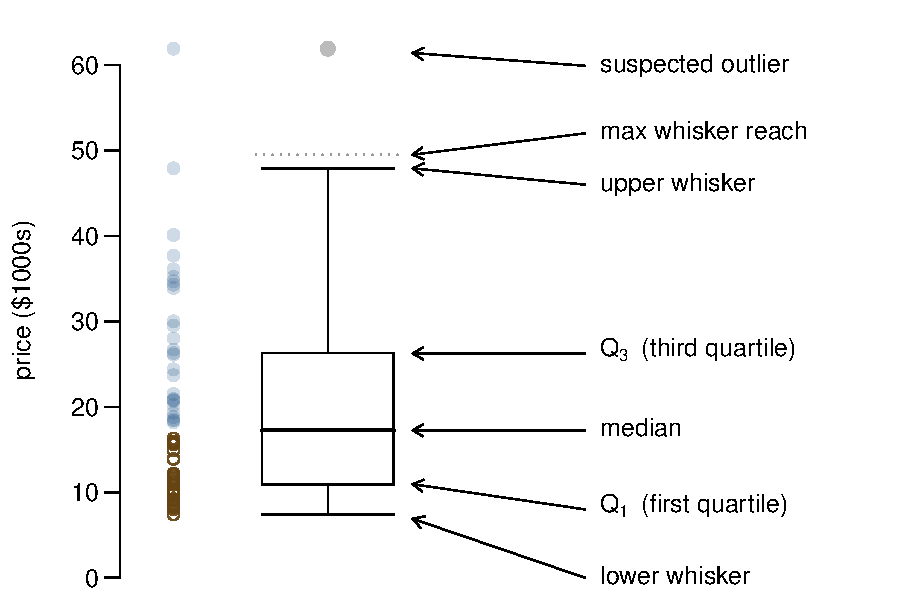
\includegraphics[height=2.5in]{ch1/boxPlotLayout/boxPlotLayout}
   \caption{Vertical dot plot and labeled box plot of the \var{price} data.}
   \label{boxPlotLayout}
\end{figure}

The first step in building a box plot is drawing a rectangle to represent the middle 50\% of the data. The total length of the box, which is the vertical distance in Figure~\ref{boxPlotLayout}, is called the \term{interquartile range} (IQR, for short). It, like the standard deviation, is one measure of variability in data. The more variable the data, the larger the standard deviation and IQR. The two boundaries of the box are called the \term{first quartile} (the $25^{th}$ percentile, i.e. 25\% of the data falls below this value) and the \term{third quartile} (the $75^{th}$ percentile), and these are often labeled $Q_1$ and $Q_3$, respectively. \\

\begin{termBox}{\tBoxTitle{Interquartile range (IQR)}
The \term{interquartile range (IQR)} is the distance
\begin{eqnarray*}
IQR = Q_3 - Q_1
\end{eqnarray*}
where $Q_1$ and $Q_3$ are the $25^{th}$ and $75^{th}$ percentiles.}
\end{termBox}

%\begin{exercise}
%The first quartile is also the $25^{th}$ \term{percentile} and the third quartile is the $75^{th}$ percentile. What does \term{percentile} mean? How many of the observations would fall below the $50^{th}$ percentile? Answers in the footnote\footnote{The  For example, the $25^{th}$ percentile is the value where 25\% of the data is below and 75\% above. The $50^{th}$ percentile is the value where half of the data is below and half above.}.
%\end{exercise}

The line splitting the box marks the \term{median}, or the ``middle'' observation in the data. There are 54 observations in the \data{Cars} data set and the $27^{th}$ and $28^{th}$ largest observations (the middle observations) are \$16,300 and \$18,200. Because this represents a tie for the middle number, the median is taken as the average of the two: \$17,250. \\

\begin{termBox}{\tBoxTitle{Median: the number in the middle}
If the data was ordered from smallest to largest, the \term{median} would be the observation right in the middle. If there are an even number of observations, two will be in the middle, and the median is taken as their average.}
\end{termBox}

\begin{exercise}
How much of the data falls between $Q_1$ and the median? How between the median and $Q_3$? Answers in the footnote\footnote{Since $Q_1$ and $Q_3$ capture the middle 50\% of the data and the median splits the middle of the data, 25\% of the data falls between $Q_1$ and the median, and another 25\% falls between the median and $Q_3$.}.
\end{exercise}

Extending out from the box, the \term{fences}\footnote{The fences are sometimes called \term{whiskers}.} attempt to capture the data outside of the box, however, their maximum reach is $1.5*IQR$. For instance, the upper fence cannot extend to the last point and must stop at $Q_3 + 1.5*IQR$ because it can reach no further, and the lower fence stops since no cars have a price lower than \$7,400. In a sense, the box is like the body of the box plot and the fences are like its arms trying to reach the rest of the data.

Any observation that lies beyond the fences is labeled with a dot. The purpose of labeling these points -- instead of just extending the fences to the minimum and maximum observed values -- is to help identify any observations that appear to be unusually distant from the rest of the data. Unusually distant observations are called \term{outliers}. In the case of the \var{price} variable, the car with price \$61,900 is a potential outlier. \\

\begin{termBox}{\tBoxTitle{Outliers are extreme}
An \term{outlier} is an observation that appears extreme relative to the rest of the data.}
\end{termBox}

Examination of data for possible outliers serves many useful purposes, including
\begin{enumerate}
\item identifying whether extreme cases are common for the variable being examined.
\item evidence of an extreme skew in the data.
\item identifying data collection or entry errors. If there was an observation listed as \$140,000, it is worth reviewing the observation to see whether it was really \$14,000.
\item providing insights into interesting phenomenon with the data.
\end{enumerate}

\begin{tipBox}{\tipBoxTitle{The use of (suspected) outliers}
The identification of outliers is not actually what is important, which is why no rigid definition for outlier is provided. What is important is to examine and take special note of \emph{suspected} outliers and why they are extreme from the rest of the data.}
\end{tipBox}

\begin{exercise}
The observation \$61,900, a suspected outlier, was found to be an accurate observation. What would such an observation suggest about the nature of vehicle prices?
\end{exercise}

\begin{exercise}
Using Figure~\vref{boxPlotLayout}, estimate the following values for \var{price} in the \data{Cars} data set: (a) $Q_1$, (b) $Q_3$, (c) IQR, and (d) the length of the upper fence. How are (c) and (d) related?
\end{exercise}

\subsection{Robust statistics}

How would sample statistics be affected if \$200,000 was observed instead of \$61,900 for the most expensive car? Or what if \$150,000 had been in the sample instead of the cheapest car at \$7,400?
\begin{center}
\includegraphics[width=6in]{ch1/carsPriceDotPlotRobustEx/carsPriceDotPlotRobustEx}
\end{center}
Sample statistics are computed under each of these scenarios in Table~\ref{robustOrNotTable}. \\
\begin{table}[ht]
\begin{center}
\begin{tabular}{l cc cc}
  \hline
& \multicolumn{2}{c}{\bf robust} & \multicolumn{2}{c}{\bf not robust} \\
scenario & median & IQR & $\bar{x}$ & $s$ \\ 
  \hline
original \var{price} data & 17.25 & 15.30 & 19.99 & 11.51 \\ 
move \$61,900 to \$200,000 & 17.25 & 15.30 & 22.55 & 26.53 \\ 
move \$7,400 to \$200,000 & 18.30 & 15.45 & 26.12 & 35.79 \\ 
   \hline
\end{tabular}
\end{center}
\caption{A comparison of how the median, IQR, mean ($\bar{x}$), and standard deviation ($s$) change when extreme observations are in play.}
\label{robustOrNotTable}
\end{table}

\begin{exercise}
Which is more affected by these changes, the mean or median? Compare also the standard deviation and IQR.
\end{exercise}

The median and IQR are called \term{robust estimates} because extreme observations have little effect on their values. The mean and standard deviation would be much more affected by changes in these extreme observations. \\

\begin{exercise}
Why doesn't the median or IQR change from the original \var{price} data to the second scenario?
\end{exercise}

\begin{exercise}
Are the extreme changes in the mean and standard deviation a fluke? Look back to how the mean and standard deviation are actually computed. Why is it that these two variables are affected by (suspected) outliers, i.e. observations that are far from the rest of the data? Compare this with how the median and IQR are computed.
\end{exercise}

\begin{exercise}
Why are robust statistics useful? If you were searching for a new car and cared about price, would you be more interested in the mean vehicle price or the median vehicle price when deciding what price you should pay for a regular car?
\end{exercise}

\section{Considering categorical data}
\label{categoricalData}

\subsection{Contingency tables}

Tables~\ref{typeDriveTrainTable} and~\ref{typeContTable} offer two perspectives of how to display categorical data in tables. These are called \term{contingency tables} and are used to organize categorical variables. The variables \var{type} and \var{driveTrain} from the \data{Cars} data set are shown in Table~\ref{typeDriveTrainTable}, where the counts represent the number of times each combination was observed. For example, there were 19 cars classified as \var{type} = \resp{small} and \var{driveTrain} = \resp{front} of the 54 cars.
\begin{table}[ht]
\begin{center}
\begin{tabular}{rrrr}
  \hline
 & front & rear & 4WD \\ 
  \hline
small &  19 &   0 &   2 \\ 
  midsize &  17 &   5 &   0 \\ 
  large &   7 &   4 &   0 \\ 
   \hline
\end{tabular}
\end{center}
\caption{A contingency table for \var{type} and \var{driveTrain}.}
\label{typeDriveTrainTable} % xtable(table(cars[,c('type','driveTrain')])[c(4,3,2),c(2,3,1)])
\end{table}

A contingency table could also be made for a single variable, as shown in Table~\ref{typeContTable}.
\begin{table}[htb]
\begin{center}
\begin{tabular}{ccc}
  \hline
small & midsize & large \\ 
  \hline
21 &  22 &  11 \\ 
   \hline
\end{tabular}
\end{center}
\caption{A contingency table only for the variable \var{type}.}
\label{typeContTable}
\end{table} % xtable(matrix(table(cars[,c('type')])[c(4,3,2)], nrow=1))

A contingency table of both \var{type} and \var{driveTrain} is shown in Table~\ref{typeDriveTrainTableTotals} with row totals and column totals added. The \term{row totals} are the sums of each row, i.e. the first row total is $19+0+2=21$. \term{Column totals} have are constructed in a similar way. \\
\begin{table}[ht]
\begin{center}
\begin{tabular}{l | ccc | r}
  \hline
 & front & rear & 4WD & total \\ 
  \hline
small &  19 &   0 & 2 & 21 \\ 
midsize &  17 &  0 & 5 & 22 \\ 
large &   7 &   4 & 0 & 11 \\ 
   \hline
total & 43 & 9 & 2 & 54 \\
   \hline
\end{tabular}
\end{center}
\caption{A contingency table for \var{type} and \var{driveTrain}. The level \resp{4WD} has been removed for instructive purposes.}
\label{typeDriveTrainTableTotals}
\end{table}

\begin{exercise}
Examine Tables~\ref{typeContTable} and~\ref{typeDriveTrainTableTotals}. Why is Table~\ref{typeContTable} redundant if Table~\ref{typeDriveTrainTableTotals} is provided?
\end{exercise}

\subsection{Bar charts and proportions}

A bar chart is the most common way to display a single categorical variable. The left panel of Figure~\ref{typeBarPlot} shows a \term{bar plot} of \var{type}. In Figure~\ref{typeBarPlot}, the bar chart was \term{standardized} by converting the counts into proportions; the \term{proportion} of cars that are \resp{small} is the number of small cars divided by the total number of cars: $21/54=0.389$. Proportions make it easy to compare the frequency of occurrence irrespective of sample size. \\
\begin{figure}[bht]
   \centering
   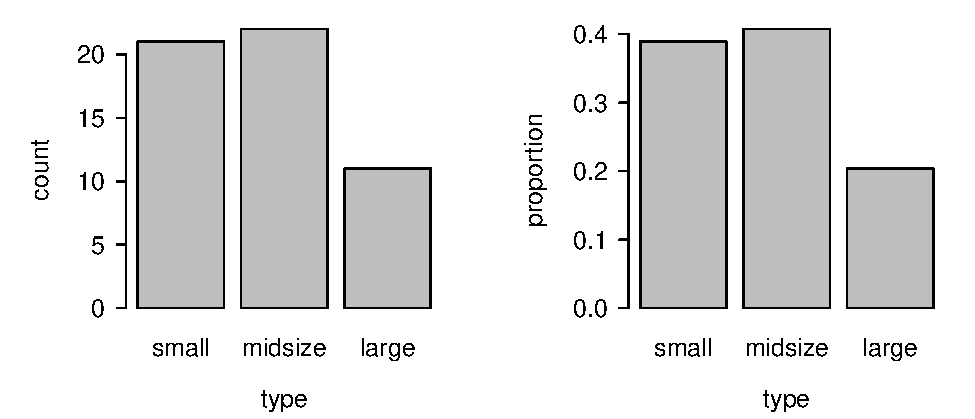
\includegraphics[height=2.3in]{ch1/typeBarPlot/typeBarPlot}
   \caption{Two bar plots of \var{type}. The first shows the counts and the second the proportions in each group.}
   \label{typeBarPlot}
\end{figure}

\begin{exercise}
Which of the following statements would be more useful to an auto executive? (1) 21 cars in our sample were of \var{type} \resp{small}. (2) 38.9\% of the cars in our sample were of \var{type} \resp{small}. Comment in the footnote\footnote{Even if the sample size (54) was provided in the first statement, the auto exec would probably just be trying to figure out the proportion in her head.}.
\end{exercise}

\begin{tipBox}{\tipBoxTitle{a proportion is like a mean}
For a particular group, assign each observation \resp{1} if it is in the group and \resp{0} if it is not. Then the proportion is the sum of these \resp{0}s and \resp{1}s divided by the sample size. This description of the proportion is useful in Chapter~\ref{foundationsForInference}.}
\end{tipBox}

If proportions are so great, why not just change Table~\ref{typeDriveTrainTableTotals} into a table of proportions? Because there is a better way. If there is a two variable contingency table, the relationship between the variables can be examined.

Table~\ref{rowPropTypeDriveTrain} shows the row proportions for Table~\ref{typeDriveTrainTableTotals}. The \term{row proportions} are computed as the counts divided by their row totals. The count 17 at the intersection of \resp{midsize} and \resp{front} is replaced by $17/22=0.773$, i.e. 17 divided by its row total, 22. So what does 0.773 represent? It corresponds to the proportion of \resp{midsize} vehicles in the sample that have front wheel drive.
\begin{table}[ht]
\begin{center}
\begin{tabular}{l | rrr | r}
  \hline
 & front & rear & 4WD & total \\ 
  \hline
small &  $19/21=0.905$ &  $0/21 = 0.000$ & $2/21 = 0.095$   & 1.000 \\ 
midsize &  $17/22 = 0.773$ &  $5/22 = 0.227$ & $0/22=0.000$ & 1.000 \\ 
large &  $7/11 = 0.636$  &   $4/11 = 0.364$  & $0/11=0.000$ & 1.000 \\ 
   \hline
total & $43/54=0.796$ & $9/54=0.167$ & $2/54 = 0.037$ &  1.000 \\
   \hline
\end{tabular}
\end{center}
\caption{The row standardized contingency table for \var{type} and \var{driveTrain}. The proportions are computed as the original counts divided by the row totals.}
\label{rowPropTypeDriveTrain}
\end{table}

A contingency table of the column proportions is computed in a similar way, where each \term{column proportion} is computed as the count divided by the corresponding column total. Table~\ref{colPropTypeDriveTrain} shows such a table. Now the proportions have a different meaning. For example, 0.442 represents the proportion of front wheel drive cars in the sample that that are small cars. \\
\begin{table}[ht]
\begin{center}
\begin{tabular}{l | rrr | r}
  \hline
 & front & rear & 4WD & total \\ 
  \hline
small &  $19/43=0.442$ &  $0/9 = 0.000$  & $2/2=1.000$ & $21/54=0.389$ \\ 
midsize &  $17/43 = 0.395$ &  $5/9 = 0.556$ & $0/2 = 0.000$ & $22/54=0.407$ \\ 
large &  $7/43 = 0.163$  &   $4/9 = 0.444$  & $0/2 = 0.000$ & $11/54=0.204$ \\ 
   \hline
total & 1.000 & 1.000 & 1.000 & 1.000 \\
   \hline
\end{tabular}
\end{center}
\caption{The column standardized contingency table for \var{type} and \var{driveTrain}. The proportions are computed as the original counts divided by the column totals.}
\label{colPropTypeDriveTrain}
\end{table}

\begin{exercise}
What does 0.364 represent in Table~\ref{rowPropTypeDriveTrain}? Answer in the footnote\footnote{0.364 represents the proportion of large cars in the sample that are rear wheel drive.}. What does 0.444 represent in Table~\ref{colPropTypeDriveTrain}?
\end{exercise}

\begin{exercise}
What does 0.796 represent in Table~\ref{rowPropTypeDriveTrain}? Answer in the footnote\footnote{0.827 represents the proportion of cars in the sample that are front wheel drive vehicles.}. What does 0.407 represent in the Table~\ref{colPropTypeDriveTrain}?
\end{exercise}

\begin{exercise} \label{weighingRowColumnProportions}
Researchers suspect \var{pop} (living location) might affect \var{sex} in the \data{possum} data set, and Table~\ref{possumPopSexContTable} is a contingency table for this data. Based on these researchers' interests, which do you think would be more interesting: row or column proportions? Answer in the footnote\footnote{The interest lies in how the \var{sex} changes based on \var{pop}. This corresponds to the row proportions here: the proportion of males/females in each location.}.
\end{exercise}

%\begin{exercise}
%Table~\ref{possumPopSexContTable} is a contingency table for the \data{possum} data set for the \var{pop} (living location) and \var{sex} variables. Which variable makes more sense as an explanatory variable? Answer in the footnote\footnote{It makes more sense for living location to affect the proportion of males to females in the population. The reverse cannot be entirely ruled out: it might be that possums migrate based on gender, although this seems less likely.}.
%\end{exercise}

%\begin{exercise} \label{weighingRowColumnProportions}
%If \var{pop} (living location) is the explanatory variable and \var{sex} the response, which do you think would be more interesting: row or column proportions? Answer in the footnote\footnote{The interest lies in how the response changes based on the explanatory variable. This corresponds to the row proportions here: the proportion of males/females in each location.% The column proportions correspond to what proportion of the sampled females and males are in each region. (If you need convincing that these are the actual meanings of the row and column proportions in these cases, construct each row and column proportion table.% You can do so in R by using the commands \rcom{prop.table(table(possum[,c('pop', 'sex')]), 1)} and \rcom{prop.table(table(possum[,c('pop', 'sex')]), 2)} after loading the data in R -- see Section~\ref{introductoryMethodsInR}.
%)}.
%\end{exercise}
\begin{table}[ht]
\begin{center}
\begin{tabular}{l cc r}
  \hline
 & f & m & total \\ 
  \hline
Vic &  24 &  22 & 46 \\ 
  other &  19 &  39 & 58 \\ 
   \hline
total & 43 & 61 & 104 \\
   \hline
\end{tabular}
\end{center}
\caption{A contingency table for \var{pop} and \var{sex} from the \data{possum} data set.}
\label{possumPopSexContTable}
\end{table}

Exercise~\exer{weighingRowColumnProportions} points out that row and column proportions are not created equal. It is important to consider each before settling on one to ensure that the most useful table is constructed.

\subsection{Mosaic plots and independence}

Tables~\ref{rowPropTypeDriveTrain} and~\ref{colPropTypeDriveTrain} can be put into a graphical form, which can be useful to examine how two categorical variables are related. Mosaic plots match the need.

The \term{mosaic plot} splits up the data according to the vertical variable, which is \var{type} in Figure~\ref{typeDriveTrainMosaicPlot}, making a rectangle for each level. The width of these three rectangles represents the number of observations in each level of \var{type}, which are the row totals in Table~\ref{typeDriveTrainTableTotals}, i.e. 19, 22, and 11. To complete the construction of the two-variable mosaic plot, each rectangle is split by the second variable, \var{driveTrain}\footnote{The two \resp{4WD} vehicles in the sample are ignored for instructive purposes. Typically all levels are included in a mosaic plot.}. For instance, the \resp{midsize} rectangle is split into two smaller rectangles. The top rectangle represents the \resp{midize}-\resp{front} cars while the bottom represents the \resp{midize}-\resp{rear} cars. Because the \var{driveTrain} splits the \var{type} variable, this is similar to how the row proportions of Table~\ref{typeDriveTrainTableTotals} split \var{driveTrain} within each level of \var{type}. In a similar way, a plot that is comparable to the column proportions of Table~\ref{typeDriveTrainTableTotals} can be constructed. This plot is shown in Figure~\ref{driveTrainTypeMosaicPlot}. \\
\begin{figure}[bth]
   \centering
   \includegraphics[height=2.4in]{ch1/typeDriveTrainMosaicPlot/typeDriveTrainMosaicPlot}
   \caption{The one-variable mosaic plot for \var{type} and the two-variable mosaic plot for both \var{type} and \var{driveTrain}.}
   \label{typeDriveTrainMosaicPlot}
\end{figure}

\begin{exercise}
What does the mosaic plot on the right of Figure~\ref{typeDriveTrainMosaicPlot} suggest about how a vehicle's \var{type} and \var{driveTrain} are related? Answer in the footnote\footnote{It appears that the larger the vehicle, the more likely it is to have a rear drive train. Do you think this result (that larger vehicles are more likely to have rear drive trains) means a vehicle being larger \emph{causes} the vehicle to have rear wheel drive? This question will be answered in Section~\ref{experiments}.}.
\end{exercise}

\begin{figure}[bth]
   \centering
   \includegraphics[height=2.3in]{ch1/driveTrainTypeMosaicPlot/driveTrainTypeMosaicPlot}
   \caption{The one-variable mosaic plot for \var{type} and the two-variable mosaic plot for both \var{type} and \var{driveTrain}.}
   \label{driveTrainTypeMosaicPlot}
\end{figure}

\begin{exercise}
Why is it that the combination \resp{rear}-\resp{small} does not have an actual rectangle? (Hint: how many cars have this combination in Table~\ref{typeDriveTrainTableTotals}.)
\end{exercise}

\begin{exercise}
Describe how the mosaic plot shown in Figure~\ref{driveTrainTypeMosaicPlot} was constructed. Answer in the footnote\footnote{First, the observations were split by \var{driveTrain} into two larger rectangles. Then the \var{type} variable splits each of these subgroups (rectangles) into their respective types.}.
\end{exercise}


%For instance, the table of row proportions is summarized by the left \term{mosaic plot} of Figure~\ref{typeDriveTrainMosaicPlot}.  This is a one-variable mosaic plot (not quite as useful as a bar plot for a single variable) then has its rectangles each split according to the second variable, \var{driveTrain}. For instance, the  en each level of \var{type} is split up by each level of \var{driveTrain}.

% The area of each rectangle in a mosaic plot is equal to the number of observations that fall in that grouping. For example, the rectangle \resp{front}-\resp{large} (the upper right rectangle) represents the cars with this combination, which is smaller than the number of



\subsection{The only pie chart you will see in this book}

While pie charts are well known, they don't do as good of a job as other charts. A \term{pie chart} is shown in Figure~\vref{carsTypePieChart} along side a bar plot. It is more difficult to compare groups in a pie chart than in a bar plot, which is why this is the first and last pie chart in this book. \\
\begin{figure}[bth]
   \centering
   \includegraphics[height=2.1in]{ch1/carsTypePieChart/carsTypePieChart}
   \caption{A pie chart and bar plot of \var{type} for the data set \data{Cars}.}
   \label{carsTypePieChart}
\end{figure}

\begin{exercise}
Using the pie chart, is it easy to tell which level, \resp{midsize} or \resp{small}, has a larger proportion in the sample? What about when using the bar plot?
\end{exercise}

\subsection{Comparing numerical data across groups}
\label{comparingAcrossGroups}

Some of the more interesting investigations can be considered by examining numerical data across groups. The methods required aren't really new. All that is required is to make a numerical plot for each group. Two convenient methods are introduced: side-by-side box plots and hollow histograms.

From the data set \data{Cars}, we break up the variable \var{price} by vehicle size (\var{type}). There are three levels of \var{type} (\resp{small}, \resp{midsize}, and \resp{large}), and each level has its own \var{price} data, as shown in Table~\ref{carsPriceSplitByTypeTable}.
\begin{table}[bt]
\begin{center}
\begin{tabular}{ cc | cc | c }
  \hline
\multicolumn{2}{c|}{\bf small} & \multicolumn{2}{c|}{\bf midsize} & {\bf large} \\ 
  \hline
15900 & 11600 & 33900 & 28000 & 20800 \\ 
9200 & 10300 & 37700 & 35200 & 23700 \\ 
11300 & 11800 & 30000 & 34300 & 34700 \\ 
12200 & 9000 & 15700 & 61900 & 18800 \\ 
7400 & 11100 & 26300 & 14900 & 18400 \\ 
10100 & 8400 & 40100 & 26100 & 29500 \\ 
8400 & 10900 & 15900 & 21500 & 19300 \\ 
12100 & 8600 & 15600 & 16300 & 20900 \\ 
8000 & 9800 & 20200 & 18500 & 36100 \\ 
10000 & 9100 & 13900 & 18200 & 20700 \\ 
8300 &  & 47900 & 26700 & 24400 \\ 
   \hline
\end{tabular}
\end{center}
\caption{The variable \var{price} split up by \var{type}.}
\label{carsPriceSplitByTypeTable}
\end{table}

The \term{side-by-side box plot} is a traditional tool for comparing across groups, and it is shown in the left panel of Figure~\vref{carsPriceByTypeSBSandHH}. This is just three box plots -- one for each \var{type} -- squished into one plotting window.
\begin{figure}[bt]
   \centering
   \includegraphics[width=5.5in]{ch1/carsPriceByTypeSBSandHH/carsPriceByTypeSBSandHH}
   \caption{Side-by-side box plot (left panel) and hollow histograms (right panel) for \var{price} where the groups are each level of \var{type}.}
   \label{carsPriceByTypeSBSandHH}
\end{figure}

Another plotting method worthy of mention is \term{hollow histograms}, which are just the histogram outlines of each group put on the same plot, as shown in the right panel of Figure~\ref{carsPriceByTypeSBSandHH}. \\

\begin{exercise} \label{comparingPriceByTypeExercise}
Use Figure~\ref{carsPriceByTypeSBSandHH} to compare the vehicle prices across groups. What do you notice about the approximate center of each group? What do you notice about the variability between groups? Is the shape relatively consistent between groups? How many \emph{prominent} modes are there for each group?
\end{exercise}

\begin{exercise}
What components of each plot do you find most useful?
\end{exercise}



\section{Observational studies and experiments}
\label{obsExp}

Beyond looking at whether variables are associated in some way, it is useful to examine the underlying nature of that association. In particular, does association always imply causation? (No.) %Beyond what the data look like, it is important to ask: how was the data collected? In this section, this question is examined carefully, and the answer to this question affects what interpretations can be drawn from the data. Not all data are collected equally!

\subsection{Explanatory and response variables}
\label{explanatoryAndResponse}

Consider the second question from page~\pageref{possibleCausationQuestionForPossums} for the \data{possum} data set:
\begin{enumerate}
\item[(2)] Will males or females, on the average, be longer?
\end{enumerate}
This question might stem from the belief that \var{sex} would affect \var{totalL} but not the reverse. If \var{sex} is suspected to affect \var{totalL}, \var{sex} is the \term{explanatory} variable and \var{totalL} is the \term{response} variable in the relationship\footnote{Sometimes the explanatory variable is called the \term{independent} variable and the response variable is called the \term{dependent} variable.}. If there are many variables, it may be possible to label a number of them as explanatory and the others as response variables, however, the discussion here will be limited to just a pair of variables. \\

\begin{tipBox}{\tipBoxTitle{Explanatory and response variables}
To identify the explanatory variable in a pair of variables, identify which of the two is suspected of affecting the other.

\hspace{6mm}\includegraphics[height=0.4in]{ch1/expResp/expResp}}
\end{tipBox}

\begin{exercise}
Would you suspect having a bigger head length might cause a change in skull width? Or could the \emph{causal} relationship be the reverse? Does it make sense to discuss causation here?
\end{exercise}

\begin{caution}{association does not imply causation}{Labeling variables as \emph{explanatory} and \emph{response} does not guarantee the relationship between the two is actually causal, even if there is some relationship identified between the two variables.}
\end{caution}

In some cases, there is no explanatory or response variable. Consider the first question from page~\pageref{possumHeadSizeQuestion}:
\begin{enumerate}
\item[(1)] If a possum has a shorter-than-average head, do you think its skull width will be smaller or larger than the average skull width?
\end{enumerate}
This question does not have an explanatory variable since it doesn't really make sense that \var{headL} would affect \var{skullW} or vice-versa, i.e. the direction is ambiguous.

%Consider the variables \var{headL} and \var{skullW} from the \data{possum} data set. A scatterplot of these variables is given in Figure~\vref{possumHeadVsSkullW}, which shows a positive association between the variables. However, it is not clear that a possum having a long skull would \emph{cause} the possum to have a wide skull, or vice versa. Instead, these variables might both be caused to vary together due to another variable such as \var{age}, \var{gender}, or an unobserved variable.

\subsection{Experiments}
\label{experiments}

An association between two variables means they are in some way connected. It would be useful to expand on this connection and say that one variable causes the other to change, however, it is not clear that is always the case. When is such a conclusion reasonable?

Consider the variables \var{pop} (living location) and \var{sex}, summarized in Table~\ref{possumPopSexContTableRowProps} using row proportions. The data suggests there might be a difference: 67\% of the sample was male for \resp{other} while only 48\% was male for \resp{Vic}. Suppose these proportions were the same in the population as in the sample, i.e. that there was a real difference in gender ratio in the two geographical regions\footnote{The biological mechanism for gender suggests the ratio should always be one male to every one female, however, the animals that actually survive might not do so in a one-to-one ratio and other factors may also play into the resulting ratio.}.
\begin{table}[ht]
\begin{center}
\begin{tabular}{rrr}
  \hline
 & f & m \\ 
  \hline
Vic & 0.52 & 0.48 \\ 
  other & 0.33 & 0.67 \\ 
   \hline
\end{tabular}
\end{center}
\caption{The row proportions of possum \var{sex} based on \var{pop} (location).}
\label{possumPopSexContTableRowProps}
\end{table}

\begin{exercise}\label{popSexExplanatoryResponse}
It may be that \var{pop} affects \var{sex} in possums. Under this setup, which variable would be the explanatory variable and which the response?
\end{exercise}

Does Exercise~\exer{popSexExplanatoryResponse} imply that living in New South Wales or Queensland  \emph{causes} a possum to be male more often than it would in Victoria? Put it another way: if possums were transported from Victoria to New South Wales or Queensland, does this actually mean their offspring is more likely to be male than if it had been born in Victoria? The data doesn't answer this \emph{causal} question.

To answer whether living location does affect gender, it would be interesting to take bunch of possums and try it out:
\begin{itemize}
\item Collect a random sample of 100 possums from Victoria (or as best a random sample as is possible).
\item Randomly split the 100 possums into two groups. Leave one group in Victoria and transport the other group to New South Wales and Queensland.
\item Observe the offspring of each group.
\end{itemize}
This setup is called an \term{experiment} because the possum locations -- the explanatory variable -- are not simply observed but are determined by random chance imposed by the researchers. If there is a big difference in these two groups again, then it would seem reasonable to conclude that living in New South Wales and Queensland actually \emph{causes} more males to be born and survive. If that difference seems to disappear or be minor, then living in New South Wales and Queensland may not cause more male possums to survive to adulthood but may just be \emph{associated} with more males surviving. \\

\begin{tipBox}{\tipBoxTitle{association $\neq$ causation}
In general, association does not imply causation, and causation can only be inferred from an experiment.}
\end{tipBox}

%An experiment offers the most straightforward way of testing the hypothesis of causality. Within the many steps of completing an experiment, there are three key concepts: \textbf{control} for lurking variables, \textbf{randomize} how the experimental groups are setup, and \textbf{replicate} the experiment many times, typically by including many subjects in the experiment. A general experiment might proceed as follows:
%\begin{enumerate}
%\item[(1)] \textbf{ID the relationship of interest.} Identify the explanatory and response variables of interest.
%\item[(2)] \textbf{ID the population, take a sample.} Identify the population of interest, and collect a random sample from this population. If the 
%\item[(3)] \textbf{Randomize.} Randomly split the sample into groups, one group for each level of the explanatory variable. For the possum study, there were two groups since there were two levels of \var{pop}: \resp{Vic} and \resp{other}.
%\item[(4)] Observe and record the response variable for each subject in each group. For the possum experiment, this meant observing the gender of each offspring in each group.
%\item[(5)] Analyze the data and look for a \emph{convincing} difference in the response variable in each group\footnote{What describes a \emph{convincing} difference will be discussed in Chapter~\ref{foundationsForInference}.}. When such a difference exists, it is (often) reasonable to conclude that there is a causal relationship.
%\end{enumerate}
%The randomization in step (3) does not guarantee bias has been eliminated in the experiment but it is a simple and important first step in reducing bias. Some forms of bias in experiments with human subjects\footnote{Human subjects are more often called \term{patients}, \term{volunteers}, or \term{study participants}.} them will be discussed in Section~\ref{biasInHumanExperiments}.

%An experiment offers the most straightforward way to test the hypothesis of causality. Within the many steps of completing an experiment, there are three key concepts: \textit{control} for lurking variables, \textit{randomize} how the experimental groups are setup, and \textit{replicate} the experiment many times, typically by including many subjects in the experiment. A general experiment might proceed as follows:
%\begin{enumerate}
%\item[(1)] Identify the explanatory and response variables of interest.
%\item[(2)] \textbf{Replicate.} Collect a random sample of many subjects from the population of interest.
%\item[(3)] \textbf{Randomize.} Randomly split the sample into groups, one group for each level of the explanatory variable. %For the possum study, there were two groups since there were two levels of \var{pop}: \resp{Vic} and \resp{other}.
%\item[(4)] Observe and record the response variable for each subject in each group. %For the possum experiment, this meant observing the gender of each offspring in each group.
%\item[(5)] Analyze the data and look for a \emph{convincing} difference in the response variable in each group\footnote{What describes a \emph{convincing} difference will be discussed in Chapter~\ref{foundationsForInference}.}. When such a difference exists, it is (often) reasonable to conclude that there is a causal relationship.
%\end{enumerate}
%The \textbf{control} step must be considered throughout. For the hypothetical possum experiment, it may be important to note which possums were siblings and include this information in the data analysis\footnote{For some species, there can be correlations in gender between siblings.}. If the experiment had human subjects\footnote{Human subjects are more often called \term{patients}, \term{volunteers}, or \term{study participants}.}, there are several strategies to control lurking variables and these will be discussed in Section~\ref{biasInHumanExperiments}.

%An experiment offers the most straightforward way of testing the hypothesis of causality. There are several steps to running an experiment:
%\begin{enumerate}
%\item[(1)] Identify the explanatory and response variables of interest. Obtain a sample of study \term{subjects} (e.g. 100 possums).
%\item[(2)] Randomly split up the study subjects into groups, one group for each level of the explanatory variable. For the possum study, there were two groups since there were two levels of \var{pop}: \resp{Vic} and \resp{other}.
%\item[(3)] Observe and record the response variable for each subject in each group. For the possum experiment, this meant observing the gender of each offspring in each group.
%\item[(4)] Analyze the data and look for a \emph{convincing} difference in the response variable in each group\footnote{What describes a \emph{convincing} difference will be discussed in Chapter~\ref{foundationsForInference}.}. When such a difference exists, it is (often) reasonable to conclude that there is a causal relationship.
%\end{enumerate}
%The randomization in step (2) does not guarantee bias has been eliminated in the experiment but it is a simple and important first step in reducing bias. Some forms of bias in experiments with human subjects\footnote{Human subjects are more often called \term{patients}, \term{volunteers}, or \term{study participants}.} them will be discussed in Section~\ref{biasInHumanExperiments}.

\begin{tipBox}{\tipBoxTitle{three experimental principles}

\textbf{Control.} Control the value of the explanatory variable in each subject or trial, and control the effects of lurking variables.

\vspace{0.3cm}
\textbf{Randomize.} Use study \term{subjects} (e.g. possums) from a random sample of the population. Subjects \emph{must} be randomly split into groups, one group for each level of the explanatory variable.

\vspace{0.3cm}
\textbf{Replicate.} Use many study subjects or run many trials.}
\end{tipBox}

Controlling lurking variables may be the most difficult part of an experiment because they are difficult to identify. For instance, it would be appropriate to control for (take into account) which possums are siblings in an analysis of the hypothetical possum experiment. In an experiment with human subjects\footnote{Human subjects are more often called \term{patients}, \term{volunteers}, or \term{study participants}.}, there are many factors to control for, and these will be discussed in more detail in Section~\ref{biasInHumanExperiments}.

If study subjects are not from a random sample of the population, additional justification is needed to extend an experiment's conclusions to the population. \\

\begin{exercise}
Describe how the three experimental principles fit into the hypothetical possum experiment.
\end{exercise}

%An experiment offers the most straightforward way to test the hypothesis of causality and there are several steps to running an experiment:
%\begin{enumerate}
%\item[(1)] Obtain a sample of \term{study subjects} (e.g. 100 possums) from the population of interest.
%\item[(2)] Randomly split up the study subjects into groups, one group for each level of the explanatory variable.
%\item[(3)] Observe and record the response variable for each subject in each group.
%\item[(4)] Analyze the data to evaluate whether there was an effect on the response based on the group.
%\end{enumerate}
%There are three key components to an experiment. First, \textit{randomization} is used to reduce bias in the data. Second, the experiment is \textit{replicated} many times by using many study subjects\footnote{In engineering applications, replications of an experiment might be called \term{replicates} instead of \textit{study subjects}.}. Lastly, lurking variables must be \textit{controlled}. Controlling lurking variables may be the most difficult part of an experiment because it may come into play in several steps. For instance, it would be appropriate to control for (take into account) which possums are siblings in an analysis of the hypothetical possum experiment. In an experiment with human subjects\footnote{Human subjects are more often called \term{patients}, \term{volunteers}, or \term{study participants}.}, there are many factors to control for, and these will be discussed in more detail in Section~\ref{biasInHumanExperiments}.

\subsection{Observational studies}

The \data{possum} data set was actually an \term{observational study} since the researchers did not randomly assign which possums lived where. Generally, data in observational studies is collected only by monitoring what occurs while experiments require the explanatory variable to be assigned for each subject by the researchers.

Inferring causal conclusions from experiments is often reasonable, however, making the same conclusions from observational data can be treacherous and is not recommended. \\

\begin{exercise} \label{sunscreenLurkingExample}
Suppose an observation study tracked sunscreen use and skin cancer and they found that the more sunscreen someone used, the more likely they were to have skin cancer (!). Does this mean sunscreen \emph{causes} skin cancer?
\end{exercise}

Exercise~\exer{sunscreenLurkingExample} has a missing variable: sun exposure. If someone is out in the sun all day, she is more likely to use sunscreen \emph{and} more likely to get skin cancer.
\begin{center}
\includegraphics[height=1.0in]{ch1/variables/sunCausesCancer}
\end{center}
It just so happens that if someone is exposed to the sun they also usually use sunscreen. Exposure to the sun is unaccounted for in the investigation, giving the incorrect impression that sunscreen causes skin cancer.

Sun exposure is what is called a \term{lurking variable}, which is a variable that is the true cause for change in the response. While one method to justify making causal conclusions from observational studies is to exhaust the search for lurking variables, there is no guarantee all lurking variables can be examined or measured.

In the same way, the \data{possum} data set is an observational study with possible lurking variables of its own, and its data cannot easily be used to make causal conclusions. \\

\begin{exercise}
There appears to be a \emph{convincing} difference in \var{sex} based on \var{pop}, however, it is unreasonable to conclude that this is a causal relationship because the data is observational. Suggest at least one lurking variables that might be the true cause for the change in \var{sex}. One lurking variable is listed in the footnote\footnote{Some genes can affect one gender more than the other. If the \resp{other} population has a gene that affects males more positively than females and this gene is less common in the \resp{Vic} population, this might explain the difference in gender ratio for each level of \var{pop}.}.
\end{exercise}

\subsection{Reducing bias in human experiments}
\label{biasInHumanExperiments}

Experiments are the gold standard for data collection but do not ensure an unbiased perspective into the cause and effect relationships in all cases. Human studies are perfect examples where bias can unintentionally arise. Let's look at a study that examines the benefits of a drug on reducing deaths from heart attacks.

Researchers wanted to examine whether a drug called sulphinpyrazone would reduce the number of deaths after heart attacks. They designed an experiment because they wanted to draw causal conclusions about the drug's effect. Study volunteers were randomly placed into two study groups. One group, the \term{treatment group}, received the drug. The other group, called the \term{control group}, did not receive any drug treatment.

Put yourself in the place of a person in the study. If you are in the treatment group, you are given a fancy new drug that you anticipate will help you. On the other hand, a person in the other group doesn't receive the drug and sits idly, hoping her participation doesn't increase her risk of death. These perspectives suggest there are actually two effects: the one of interest is the effectiveness of the drug and the second is an emotional effect that is difficult to quantify.

Researchers aren't interested in this emotional effect, which might bias the study. Instead, researchers do not want patients to know which group they are in. When researchers keep the patients in the dark about their treatment, the study is said to be \term{blind}. But there is one problem: if a patient doesn't receive a treatment, she will know she is in the control group. The solution to this problem is to give fake treatments to patients in the control group. A fake treatment is called a \term{placebo}, and an effective placebo is the key to making a study truly blind. A classic example of a placebo is a sugar pill that is made to look like the actual treatment pill. Often times, a placebo results in a slight but real improvement in patients. This often positive effect has been dubbed the \term{placebo effect}.

% Researchers aren�t interested in this emotional effect, which might bias the study, although it is not entirely obvious which way the bias would be. There are two methods to reduce or eliminate the bias. First, give the patients in the control group a fake treatment, which is called a placebo. Usually this is just a sugar pill that looks like the real drug. Then, for this placebo to eliminate this emotional effect, don�t tell any of the patients if they are receiving the real drug or the placebo so all are under the same emotional condition. In this setup, the study is said to be \term{blind} since no patients know their treatment. Findings suggest patients in control groups respond differently when the study is blinded to when it is not, and this effect  that the placebo is eliminating is aptly named the \term{placebo effect}.

The patients are not the only ones who should be blinded: doctors and researchers can accidentally bias a study. When a doctor knows a patient has been given the real treatment, she might inadvertently give that patient more attention or care than a patient that she knows is on the placebo. To guard against this bias (which again has been found to have a measurable effect in some instances), most modern studies employ a \term{double-blind} setup where doctors or researchers who interact with patients are, just like the patients, unaware of who is or is not receiving the treatment\footnote{There are always some researchers involved in the study who do know which patients are receiving which treatment, however, they do not have interactions with the patients and do not tell the \emph{blinded} doctors who is receiving which treatment.}.

\subsection{Variability within data (optional)}
\label{variabilityWithinData}

The study examining the effect of sulphinpyrazone was double-blinded, and the results are given in Table~\ref{sulphinpyrazoneResults}. Do these results mean the drug was effective at reducing deaths? In the observed groups, a smaller proportion of individuals died in the treatment group than the control group (0.056 versus 0.081), however, it is unclear whether that difference is \emph{convincing evidence} that the drug is effective. \\
\begin{table}[ht]
\begin{center}
\begin{tabular}{l cc}
  \hline
		& lived 	& died	 \\ 
  \hline
drug 		& 692    	& 41     	 \\ 
placebo 	& 682    	& 60     	 \\ 
   \hline
\end{tabular}
\end{center}
\caption{The row proportions of possum \var{sex} based on \var{pop} (location).}
\label{sulphinpyrazoneResults}
\end{table}

\begin{example}{Suppose there had been only 42 deaths in the placebo group. Would this be convincing evidence that the drug was effective?} \label{42PlaceboDeaths}
The proportion is still in favor of the drug (0.056 versus 0.057), however, this minor difference is really not very convincing. It is not as though the sample proportion is exactly equal to what will happen with all heart attack victims but the sample only \emph{estimates} what will happen.
\end{example}

Example~\exam{42PlaceboDeaths} is a reminder that the population will not perfectly reflect the sample. It is true that the samples are pretty large, however, it is unclear what difference is needed for this evidence to be convincing.

In Chapters~\ref{foundationsForInference} and~\ref{classicalInference}, methods for identifying what is and is not convincing evidence will be discussed in detail. Until then, a larger statistical foundation is needed to understand and make competent use of those methods.

%\section{Two more data collection procedures}

%\subsection{Why go beyond simple random sampling?}



%\subsection{Cluster sampling}



%\subsection{Stratified sampling}

